\chapter{Введение}
Целью данной работы является изучение методики и технологии синтеза аппаратных устройств ускорения вычислений по описаниям на языках высокого уровня. В ходе лабораторной работы рассматривается маршрут проектирования устройств, представленных в виде синтаксических конструкций ЯВУ C/C++, изучаются принципы работы IDE Xilinx Vitis HLS и методика анализа и отладки устройств. 


В ходе работы необходимо разработать ускоритель вычислений по индивидуальному заданию, разработать код для тестирования ускорителя, реализовать ускоритель с помощью средств высоко уровненного синтеза, выполнить его отладку.

Для достижения данной цели необходимо выполнить следующие задачи:
\begin{enumerate}
	\item Разработать ускоритель вычислений по индивидуальному заданию;
	\item Разработать код для тестирования ускорителя, реализовать ускоритель с помощью средств высоко уровненного синтеза;
	\item Выполнить отладку реализованного ускорителя.
\end{enumerate}

\chapter{Практическая часть}

\begin{lstlisting}[label=some-code-1,caption=Листинг неоптимизированного кода]
extern "C" {
void var002_no_prragmas(int* c, const int* a, const int* b, const int len) {
    for (int i = 0; i < len; i+=2) {
          if (b[i] > a[i]) {
               c[i] = b[i];
          } else {
               c[i]= a[i];
          }
    }
    for (int i = 1; i < len; i+=2) {
          if (b[i] < a[i]) {
               c[i] = b[i];
          } else {
               c[i]= a[i];
          }
    }
}
}
\end{lstlisting}

\begin{lstlisting}[label=some-code-1,caption=Листинг кода с конвейерной организацией]
extern "C" {
void var002_pipelined(int* c, const int* a, const int* b, const int len) {
    for (int i = 0; i < len; i+=2) {
#pragma HLS PIPELINE
          if (b[i] > a[i]) {
               c[i] = b[i];
          } else {
               c[i]= a[i];
          }
    }
    for (int i = 1; i < len; i+=2) {
          if (b[i] < a[i]) {
               c[i] = b[i];
          } else {
               c[i]= a[i];
          }
    }
}
}
\end{lstlisting}

\begin{lstlisting}[label=some-code-1,caption=Листинг кода с развёрткой]
extern "C" {
void var002_unrolled(int* c, const int* a, const int* b, const int len) {
    for (int i = 0; i < len; i+=2) {
#pragma HLS UNROLL factor = 2
          if (b[i] > a[i]) {
               c[i] = b[i];
          } else {
               c[i]= a[i];
          }
    }
    for (int i = 1; i < len; i+=2) {
#pragma HLS UNROLL factor = 2
          if (b[i] < a[i]) {
               c[i] = b[i];
          } else {
               c[i]= a[i];
          }
    }
}
}
\end{lstlisting}

\begin{lstlisting}[label=some-code-1,caption=Листинг кода с развёрткой и конвейерной организацией]
extern "C" {
void var002_pipe_unroll(int* c, const int* a, const int* b, const int len) {
    for (int i = 0; i < len; i+=2) {
#pragma HLS PIPELINE
#pragma HLS UNROLL factor = 2
          if (b[i] > a[i]) {
               c[i] = b[i];
          } else {
               c[i]= a[i];
          }
    }
    for (int i = 1; i < len; i+=2) {
#pragma HLS UNROLL factor = 2
          if (b[i] < a[i]) {
               c[i] = b[i];
          } else {
               c[i]= a[i];
          }
    }
}
}

\end{lstlisting}


\chapter{Результаты сборки и отладки в режиме Emulation SW}

\begin{figure}[ph!]
	\center{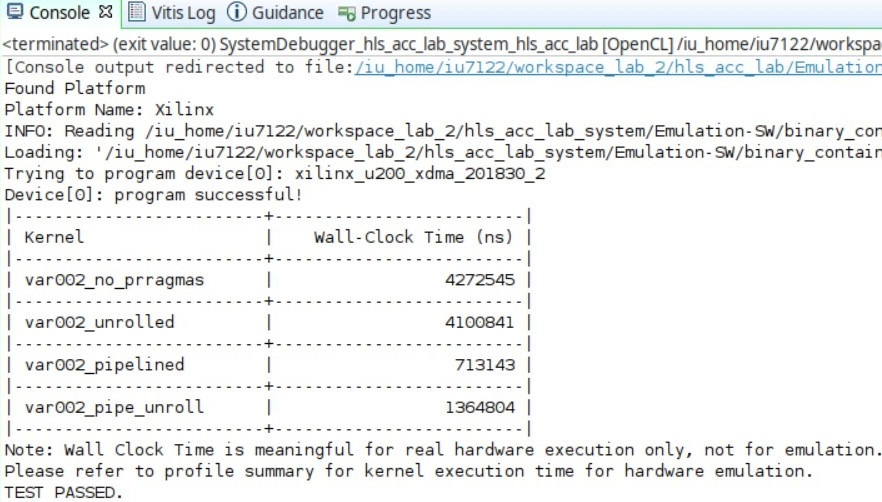
\includegraphics[scale=0.7]{emulation sw}}
	\caption{Результат работы программы}
\end{figure}

\newpage

\chapter{Результаты сборкии отладки в режиме Emulation HW}

\begin{figure}[ph!]
	\center{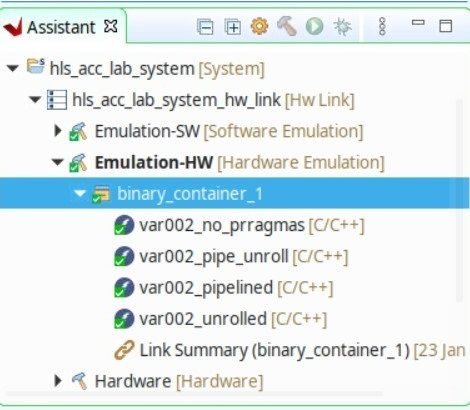
\includegraphics[scale=0.5]{emulation hw assistant}}
	\caption{Assistant View}
\end{figure}

\begin{figure}[ph!]
	\center{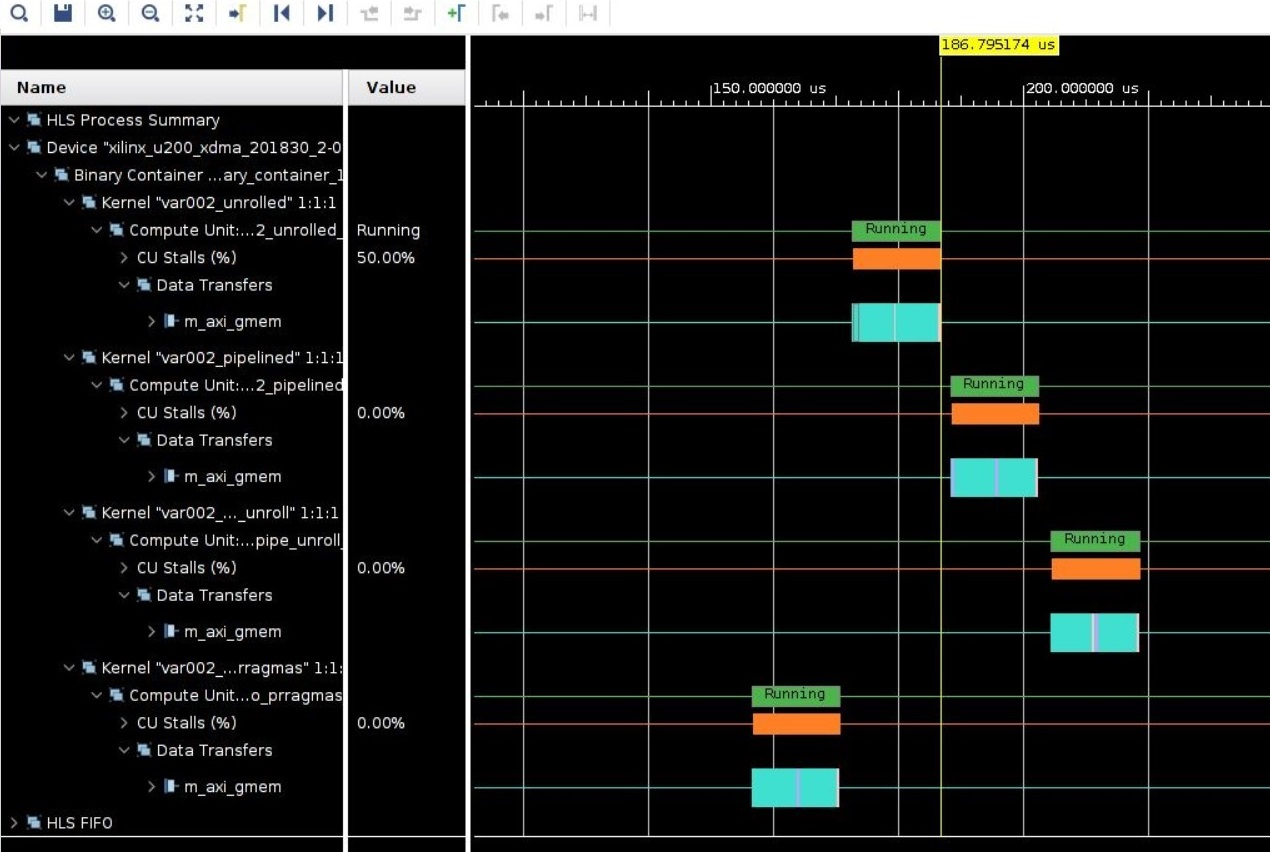
\includegraphics[scale=0.5]{emulation hw kernel work}}
	\caption{Окно внутрисхемового отладчика Vivado}
\end{figure}

\begin{figure}[ph!]
	\center{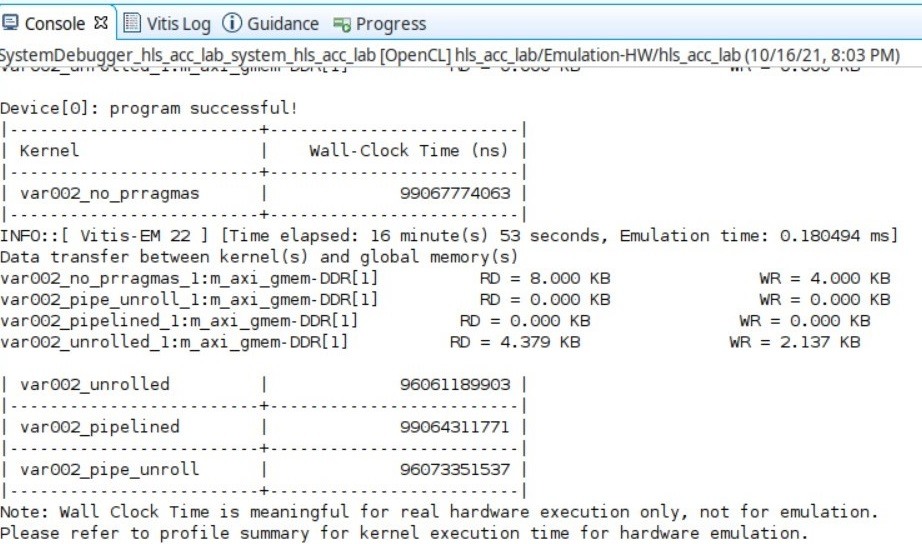
\includegraphics[scale=0.7]{emulation hw test results}}
	\caption{Результат работы программы}
\end{figure}

\newpage

\chapter{Результаты сборкии отладки в режиме Hardware}

\begin{figure}[ph!]
	\center{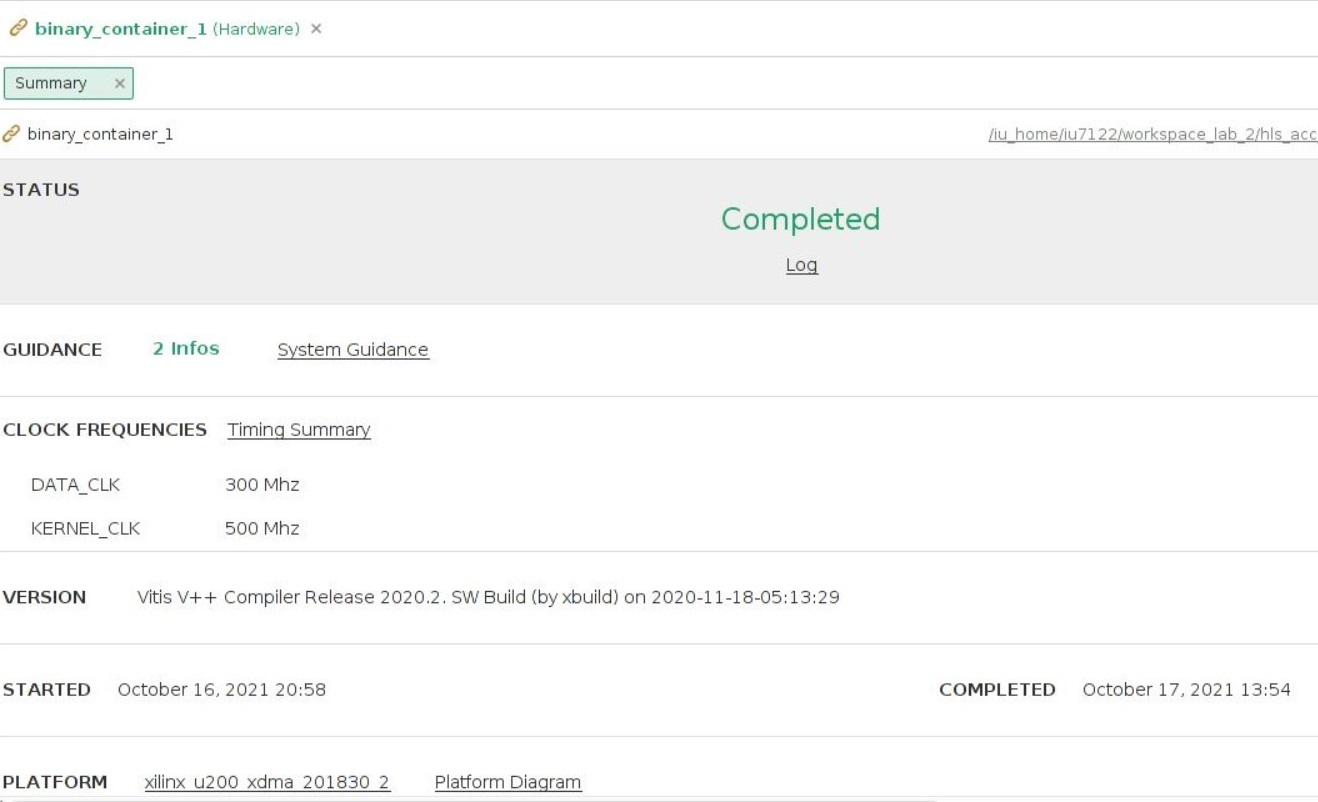
\includegraphics[scale=0.5]{hw summary 1}}
	\caption{Содержимое вкладки Summary часть 1}
\end{figure}

\begin{figure}[ph!]
	\center{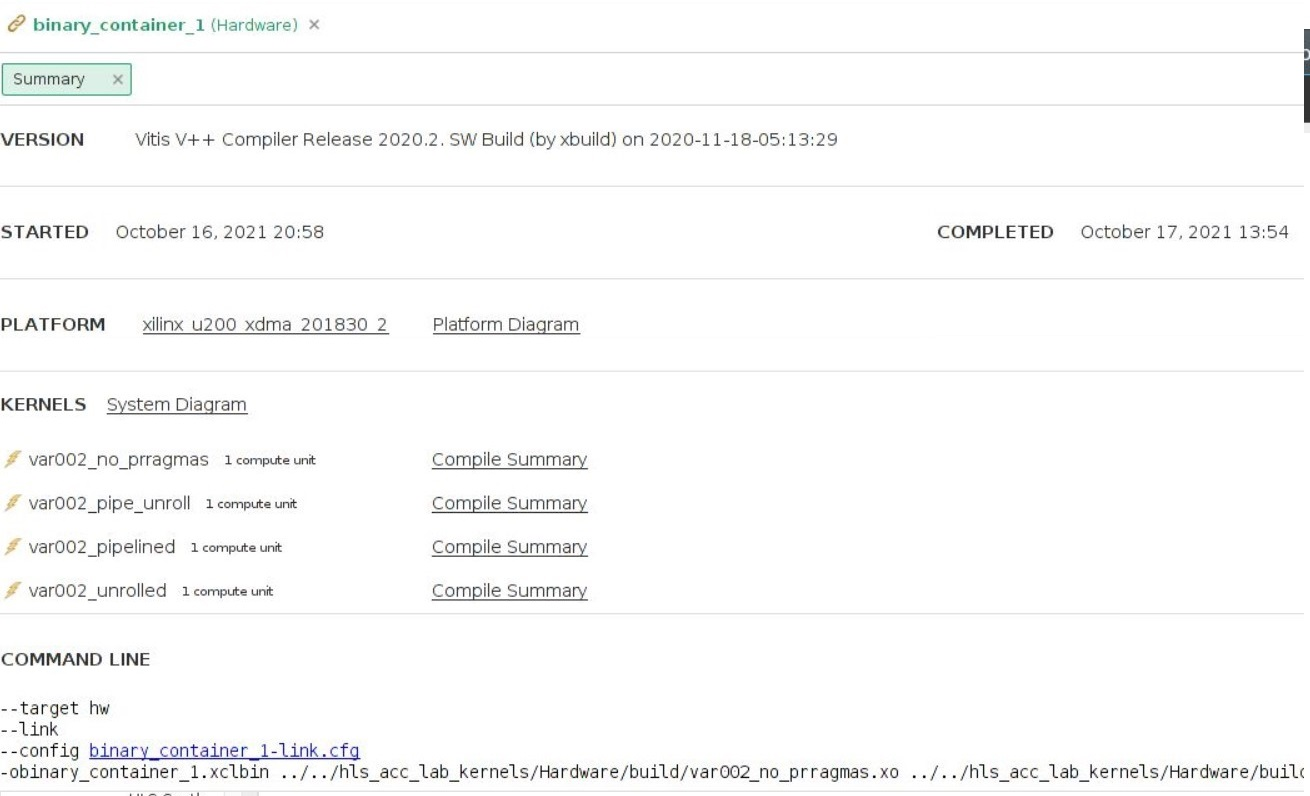
\includegraphics[scale=0.5]{hw summary 2}}
	\caption{Содержимое вкладки Summary часть 2}
\end{figure}

\begin{figure}[ph!]
	\center{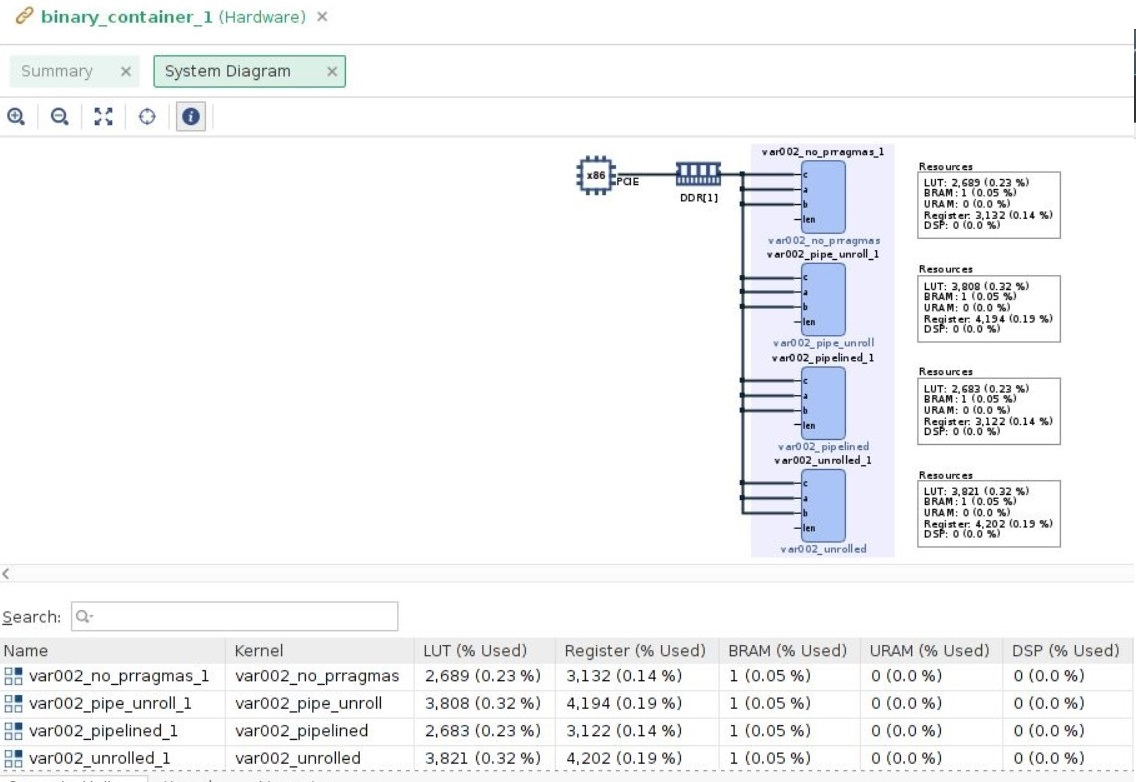
\includegraphics[scale=0.5]{hw system diagram}}
	\caption{Содержимое вкладки System Diagram}
\end{figure}

\begin{figure}[ph!]
	\center{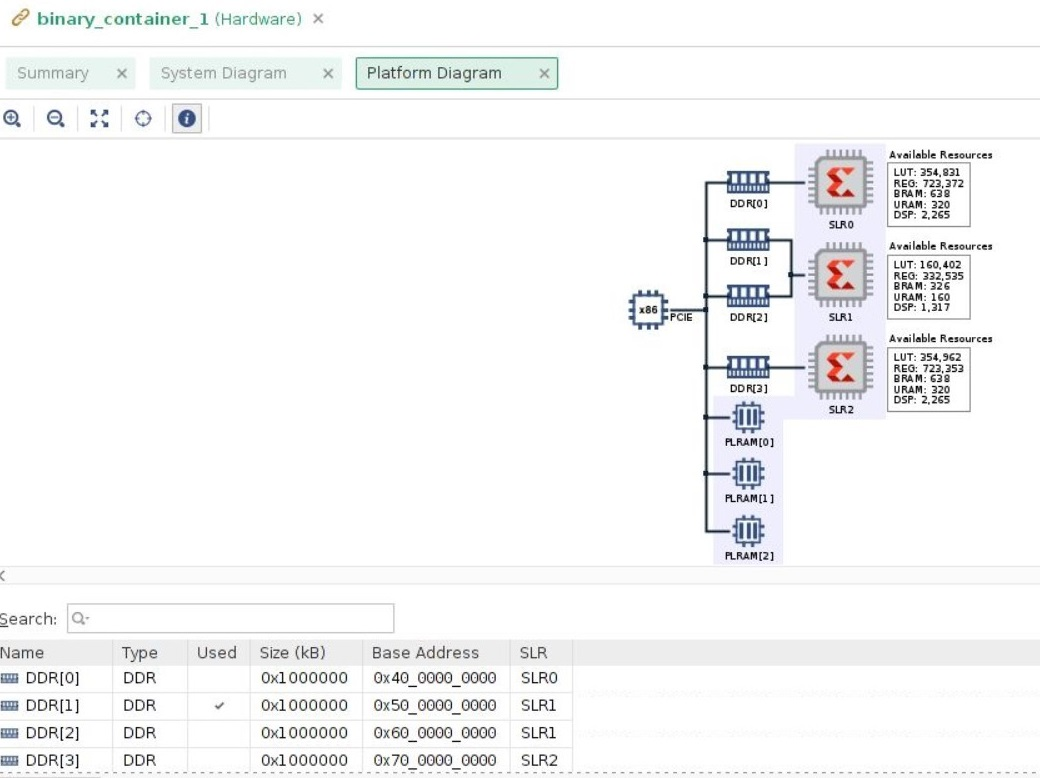
\includegraphics[scale=0.5]{hw platform}}
	\caption{Содержимое вкладки Platform Diagram}
\end{figure}

\begin{figure}[ph!]
	\center{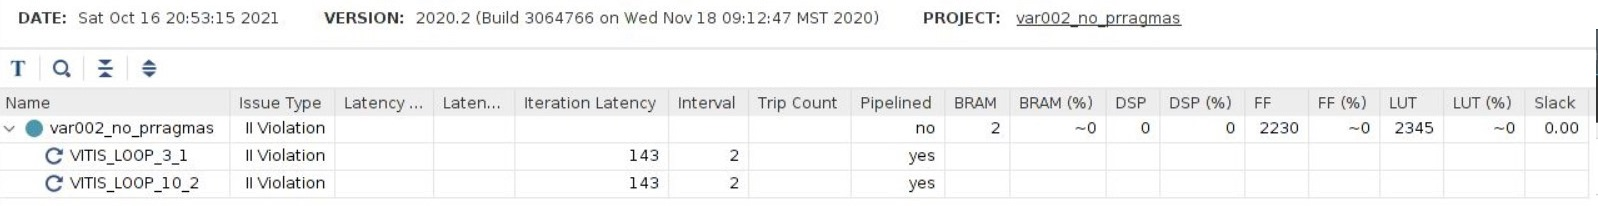
\includegraphics[scale=0.5]{HLS no params}}
	\caption{HLS no params}
\end{figure}

\begin{figure}[ph!]
	\center{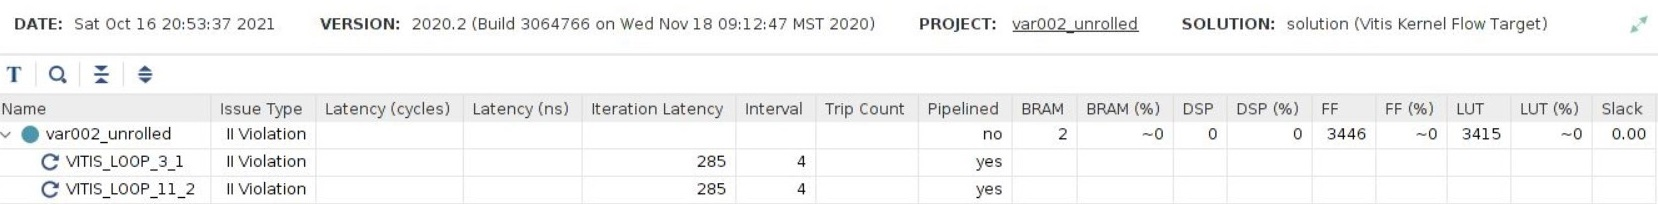
\includegraphics[scale=0.5]{HLS unroll}}
	\caption{HLS unroll}
\end{figure}

\begin{figure}[ph!]
	\center{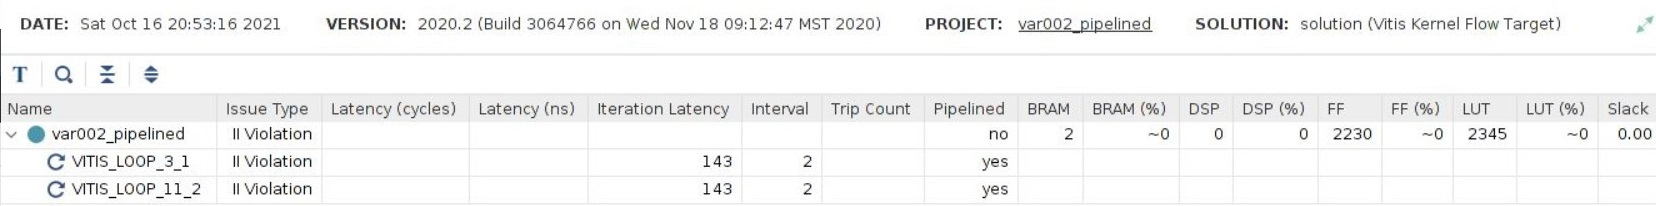
\includegraphics[scale=0.5]{HLS pipe}}
	\caption{HLS pipe}
\end{figure}

\begin{figure}[ph!]
	\center{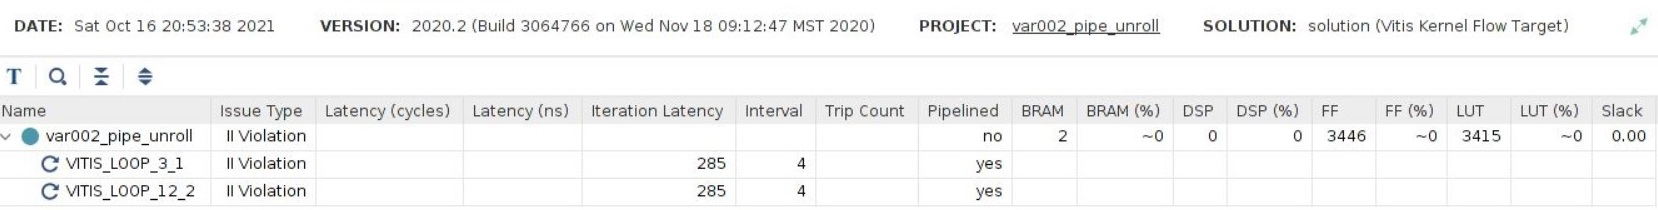
\includegraphics[scale=0.5]{HLS pipe unroll}}
	\caption{HLS pipe unroll}
\end{figure}

\begin{figure}[ph!]
	\center{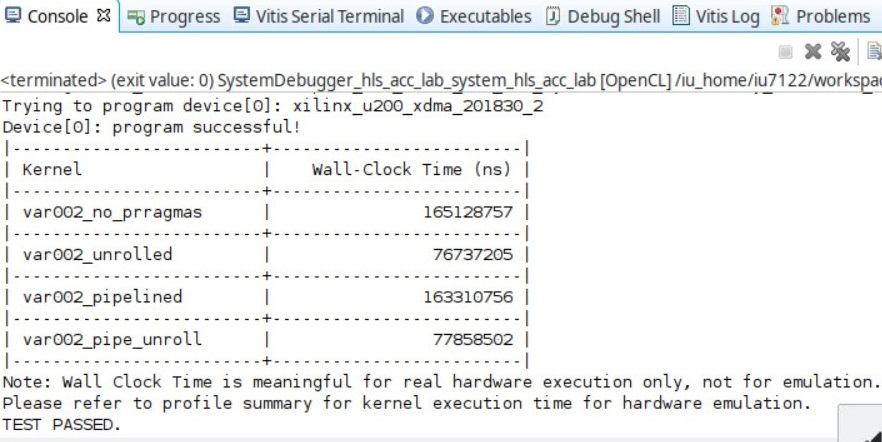
\includegraphics[scale=0.7]{hw results}}
	\caption{Результаты работы программы}
\end{figure}

\newpage

\chapter{Вывод}
В ходе лабораторной работы были изучены архитектура гетерогенных вычислительных систем и технологии разработки ускорителей вычислений на базе ПЛИС фирмы Xilinx. Была выполнена генерация ядра ускорителя с последующим синтезом, сборкой и тестированием бинарного модуля ускорителя.

В результате сборки проекта было выяснено, что использование оптимизаций приводит к реальному повышению быстродействия работы программы. Однако следует отметить, что в режиме программной эмуляции выигрыш получился наиболее существенным (до 3-х раз), а в режимах аппаратной эмуляции и аппаратного исполнения ускорение осталось, но оно не настолько существенное (до 5-10\%). Это можно объяснить тем, что возможно объем тестирования был недостаточным и небольшая выборка данных не позволяет получить наиболее точные результаты, также ввиду большой загруженности удаленного сервера и разного количества пользователей на нем, тестирование происходило не в равных условиях.
